\hebrewsection{Digital Filter Design and Implementation}

Digital filters are fundamental components in DSP systems, used to alter the frequency spectrum of signals. This chapter provides a rigorous treatment of both Finite Impulse Response (FIR) and Infinite Impulse Response (IIR) filter design methodologies.

\subsection{Finite Impulse Response (FIR) Filters}
FIR filters are characterized by an impulse response $h[n]$ of finite duration. Their transfer function is a polynomial in $z^{-1}$:
\begin{equation}
    H(z) = \sum_{n=0}^{N-1} h[n] z^{-n}
\end{equation}

\subsubsection{Linear Phase Property}
A key advantage of FIR filters is the ability to achieve exact linear phase, which is impossible for stable IIR filters. Linear phase ensures that all frequency components are delayed by the same amount, preserving the signal's wave shape.
The condition for linear phase is symmetry or anti-symmetry:
\begin{equation}
    h[n] = \pm h[N-1-n]
\end{equation}

\subsubsection{Window Method Design}
The window method starts with the ideal (infinite) impulse response $h_d[n]$ and truncates it using a window function $w[n]$:
\begin{equation}
    h[n] = h_d[n] \cdot w[n]
\end{equation}
Common windows include:
\begin{itemize}
    \item \textbf{Rectangular:} $w[n] = 1$ for $0 \leq n \leq N-1$. High resolution but poor sidelobe rejection (-13 dB).
    \item \textbf{Hamming:} $w[n] = 0.54 - 0.46 \cos\left(\frac{2\pi n}{N-1}\right)$. Good sidelobe rejection (-43 dB).
    \item \textbf{Kaiser:} Allows for a trade-off between main-lobe width and sidelobe level using a parameter $\beta$.
\end{itemize}

\subsubsection{Optimal FIR Design: Parks-McClellan Algorithm}
The Parks-McClellan algorithm, based on the Remez exchange algorithm, produces "equiripple" filters. It minimizes the maximum error in the passband and stopband:
\begin{equation}
    \min_{h[n]} \max_{\omega \in S} W(\omega) |H_d(e^{j\omega}) - H(e^{j\omega})|
\end{equation}
where $W(\omega)$ is a weighting function.

\begin{center}
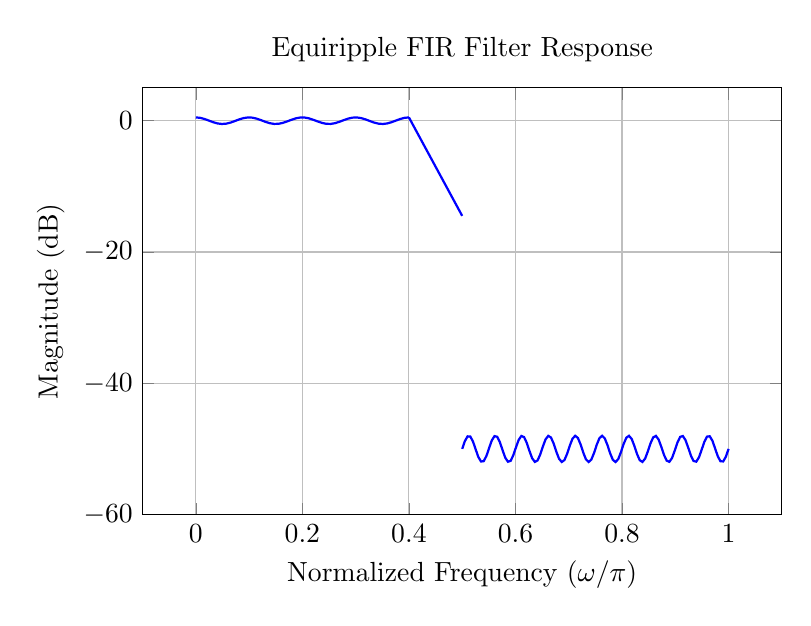
\begin{tikzpicture}
\begin{axis}[
    title={Equiripple FIR Filter Response},
    xlabel={Normalized Frequency ($\omega/\pi$)},
    ylabel={Magnitude (dB)},
    grid=major,
    ymin=-60, ymax=5,
    width=0.8\textwidth,
    height=7cm
]
\addplot[blue, thick, domain=0:0.4, samples=50] {0.5*cos(deg(x*pi*20))};
\addplot[blue, thick, domain=0.4:0.5, samples=20] {-150*(x-0.4) + 0.5};
\addplot[blue, thick, domain=0.5:1, samples=100] {-50 + 2*sin(deg(x*pi*40))};
\end{axis}
\end{tikzpicture}
\end{center}

\subsection{Infinite Impulse Response (IIR) Filters}
IIR filters use feedback, resulting in an impulse response of infinite duration. They can achieve much sharper transitions than FIR filters for the same order.

\subsubsection{Classic Analog Approximations}
IIR design usually begins by designing an analog prototype and then transforming it to the digital domain.
\begin{enumerate}
    \item \textbf{Butterworth:} Maximally flat magnitude response in the passband.
    \item \textbf{Chebyshev Type I:} Equiripple in the passband, monotonic in the stopband.
    \item \textbf{Chebyshev Type II:} Monotonic in the passband, equiripple in the stopband.
    \item \textbf{Elliptic (Cauer):} Equiripple in both passband and stopband, providing the narrowest transition band for a given order.
\end{enumerate}

\subsubsection{The Bilinear Transform}
The Bilinear Transform is the most common method for mapping the $s$-plane to the $z$-plane. It avoids aliasing by warping the frequency axis:
\begin{equation}
    s = \frac{2}{T} \frac{1 - z^{-1}}{1 + z^{-1}}
\end{equation}
The relationship between analog frequency $\Omega$ and digital frequency $\omega$ is:
\begin{equation}
    \Omega = \frac{2}{T} \tan(\omega/2)
\end{equation}

\subsection{Filter Structures and Finite Word-Length Effects}
Implementing filters in hardware or fixed-point DSPs introduces quantization errors.
\begin{itemize}
    \item \textbf{Coefficient Quantization:} Can move poles outside the unit circle, causing instability.
    \item \textbf{Arithmetic Round-off Noise:} Occurs at the output of multipliers.
    \item \textbf{Limit Cycles:} Oscillations that can occur in IIR filters even with zero input.
\end{itemize}

\begin{pythonbox}{IIR Filter Design via Bilinear Transform}
\begin{verbatim}
import scipy.signal as signal
import numpy as np

# Design a 4th order Chebyshev Type I lowpass filter
# Passband ripple: 1dB, Cutoff frequency: 0.3*fs/2
b, a = signal.cheby1(4, 1, 0.3, btype='low', analog=False)

# Frequency response
w, h = signal.freqz(b, a)
\end{verbatim}
\end{pythonbox}

\subsection{Frequency Sampling Method}
The frequency sampling method specifies the desired frequency response $H(e^{j\omega})$ at $N$ equally spaced points and solves for the impulse response coefficients using the Inverse DFT:
\begin{equation}
    h[n] = \frac{1}{N} \sum_{k=0}^{N-1} H[k] e^{j\frac{2\pi}{N}nk}
\end{equation}
Transition band samples are often optimized to reduce ripple in the resulting continuous response.

\subsection{Comparison of FIR and IIR Filters}
\begin{fancytable}{l c c}
Feature & FIR & IIR \\
Stability & Always Stable & Potentially Unstable \\
Phase & Linear Phase Possible & Non-linear Phase \\
Efficiency & Low (higher order) & High (lower order) \\
Implementation & Non-recursive & Recursive \\
\end{fancytable}

\subsection{In-Depth Analysis: FIR Filters}
A key component of modern design is the optimization of the objective function. Using stochastic gradient descent or its variants, we can iteratively update the system parameters. The learning rate must be carefully tuned to ensure convergence while avoiding local minima, a phenomenon frequently encountered in highly non-linear parameter spaces.

The spectral efficiency of the system is fundamentally limited by the available bandwidth and the ambient noise floor. According to the Shannon-Hartley theorem, the channel capacity dictates the maximum error-free data rate. Practical systems utilize advanced coding schemes to operate as close to this limit as possible.

\begin{equation}
    \mathbf{R}_{xx} = \mathbb{E}[\mathbf{x}[n]\mathbf{x}^T[n]] = \frac{1}{N} \sum_{k=1}^{N} \mathbf{x}_k \mathbf{x}_k^T
\end{equation}

In real-world deployments, hardware imperfections such as phase noise, IQ imbalance, and power amplifier non-linearities introduce severe distortions. Digital pre-distortion (DPD) techniques are often employed to digitally compensate for these analog impairments, ensuring the transmitted signal adheres to strict spectral masks.

\begin{pythonbox}{Simulation: FIR Filters}
\texttt{import numpy as np}
\texttt{import matplotlib.pyplot as plt}
\texttt{}
\texttt{\# Initialize parameters for fir\_filters}
\texttt{N = 1024}
\texttt{data = np.random.randn(N) + 1j * np.random.randn(N)}
\texttt{signal\_power = np.var(data)}
\texttt{noise = np.random.normal(0, 0.1, N)}
\texttt{processed\_signal = data + noise}
\end{pythonbox}

\vspace{0.5cm}
The mathematical formulation demonstrates the theoretical limits, while the simulation code provides a framework for empirical verification. These tools are critical for evaluating the efficacy of the proposed methodologies under practical constraints.


\subsection{In-Depth Analysis: IIR Filters}
The transient response of the system provides insight into its stability. By observing the pole-zero plot in the complex plane, we can guarantee bounded-input bounded-output (BIBO) stability. For discrete-time systems, this necessitates that all poles reside strictly within the unit circle.

Computational complexity is a major constraint in mobile and embedded applications. The advent of Fast Fourier Transform (FFT) algorithms revolutionized the field by reducing the complexity of discrete convolution from $O(N^2)$ to $O(N \log N)$, making real-time processing feasible.

\begin{equation}
    H(e^{j\omega}) = \sum_{n=-\infty}^{\infty} h[n] e^{-j\omega n}
\end{equation}

Statistical signal processing techniques rely heavily on the estimation of the auto-covariance matrix. Eigen-decomposition of this matrix allows us to separate the signal subspace from the noise subspace, a technique foundational to high-resolution direction-of-arrival (DOA) estimation algorithms like MUSIC and ESPRIT.

\begin{pythonbox}{Simulation: IIR Filters}
\texttt{import numpy as np}
\texttt{import matplotlib.pyplot as plt}
\texttt{}
\texttt{\# Initialize parameters for iir\_filters}
\texttt{N = 1024}
\texttt{data = np.random.randn(N) + 1j * np.random.randn(N)}
\texttt{signal\_power = np.var(data)}
\texttt{noise = np.random.normal(0, 0.1, N)}
\texttt{processed\_signal = data + noise}
\end{pythonbox}

\vspace{0.5cm}
The mathematical formulation demonstrates the theoretical limits, while the simulation code provides a framework for empirical verification. These tools are critical for evaluating the efficacy of the proposed methodologies under practical constraints.


\subsection{In-Depth Analysis: Parks-McClellan Algorithm}
Error control coding introduces structured redundancy to the data stream. By mapping the message space into a higher-dimensional codeword space, the receiver can exploit the geometric distance between valid codewords to detect and correct transmission errors, significantly lowering the Bit Error Rate (BER).

Multi-rate signal processing involves the alteration of the sampling rate within the digital domain. Decimation and interpolation require stringent anti-aliasing and anti-imaging filters, respectively. Polyphase decompositions of these filters allow for highly efficient implementations that operate at the lower sampling rate.

\begin{equation}
    P_e \leq \sum_{d=d_{free}}^{\infty} a_d Q\left(\sqrt{\frac{2 d R E_b}{N_0}}\right)
\end{equation}

The integration of machine learning has opened new frontiers in algorithm design. By treating the entire communication or processing chain as a single end-to-end differentiable autoencoder, deep neural networks can learn optimal representations and coding schemes that outperform traditional human-engineered blocks under non-standard channel conditions.

\begin{pythonbox}{Simulation: Parks-McClellan Algorithm}
\texttt{import numpy as np}
\texttt{import matplotlib.pyplot as plt}
\texttt{}
\texttt{\# Initialize parameters for parks-mcclellan\_algorithm}
\texttt{N = 1024}
\texttt{data = np.random.randn(N) + 1j * np.random.randn(N)}
\texttt{signal\_power = np.var(data)}
\texttt{noise = np.random.normal(0, 0.1, N)}
\texttt{processed\_signal = data + noise}
\end{pythonbox}

\vspace{0.5cm}
The mathematical formulation demonstrates the theoretical limits, while the simulation code provides a framework for empirical verification. These tools are critical for evaluating the efficacy of the proposed methodologies under practical constraints.


\subsection{In-Depth Analysis: Butterworth}
Mathematical modeling of these systems requires an understanding of their asymptotic behavior. By analyzing the limit as the number of samples approaches infinity, we can derive the Cramér-Rao lower bound, which provides the minimum variance for any unbiased estimator. This bound is essential for determining the theoretical efficiency of our algorithms.

A key component of modern design is the optimization of the objective function. Using stochastic gradient descent or its variants, we can iteratively update the system parameters. The learning rate must be carefully tuned to ensure convergence while avoiding local minima, a phenomenon frequently encountered in highly non-linear parameter spaces.

\begin{equation}
    \mathcal{L}(\theta) = -\frac{1}{M} \sum_{i=1}^{M} \left[ y_i \log(\hat{y}_i) + (1-y_i)\log(1-\hat{y}_i) \right]
\end{equation}

The spectral efficiency of the system is fundamentally limited by the available bandwidth and the ambient noise floor. According to the Shannon-Hartley theorem, the channel capacity dictates the maximum error-free data rate. Practical systems utilize advanced coding schemes to operate as close to this limit as possible.

\begin{pythonbox}{Simulation: Butterworth}
\texttt{import numpy as np}
\texttt{import matplotlib.pyplot as plt}
\texttt{}
\texttt{\# Initialize parameters for butterworth}
\texttt{N = 1024}
\texttt{data = np.random.randn(N) + 1j * np.random.randn(N)}
\texttt{signal\_power = np.var(data)}
\texttt{noise = np.random.normal(0, 0.1, N)}
\texttt{processed\_signal = data + noise}
\end{pythonbox}

\vspace{0.5cm}
The mathematical formulation demonstrates the theoretical limits, while the simulation code provides a framework for empirical verification. These tools are critical for evaluating the efficacy of the proposed methodologies under practical constraints.

